\section{Auswertung}
\label{sec:Auswertung}

\subsection{Bestimmung der Winkelrichtgröße und des Eigenträgheitsmoments der Drillachse}


\subsubsection{Winkelrichtgröße}

Die Winkelrichtgröße D lässt sich mithilfe der Gleichungen \ref{eq:fa1} und \ref{eq:fa3} berechnen.
Im Versuch stehen Kraftarm $\vec{r}$ und Kraft $\vec{F}$ senkrecht zueinander, wodurch der Betrag
von Gleichung \ref{eq:fa1} 
zu
\begin{equation}
    M = F \cdot r
    \label{eq:ae1}
\end{equation}
\noindent
wird. Werden nun \ref{eq:fa3} und \ref{eq:ae1} gleichgesetzt und nach D umgestellt, ergibt sich
die Gleichungen
\begin{equation}
    D = \frac{F\cdot r}{\phi}.
    \label{eq:ae2}
\end{equation}
\noindent
Mit den Werten aus der Tabelle \ref{tab:a1}, der Formel \ref{eq:ae2} und den allgemeinen Formeln 
für den Mittelwert
\begin{equation}
    \bar{x} = \frac{1}{N} \sum_{n=1}^N x_n 
    \label{eq:ae3}
\end{equation}
\noindent
und der Standartabweichung
\begin{equation}
    \Delta x = \sqrt{\frac{1}{N(N-1)} \sum_{n=1}^N (x_n - \bar{x})^2}
    \label{eq:std}
\end{equation}
\noindent
ergibt sich für die Winkelrichtgröße der Wert D = $(0.017027 \pm 0.001539)\,$Nm.

\begin{table}[H]
\normalsize

\centering
\sisetup{table-format=4.0}
\begin{tabular}{c c}
\toprule
    $\phi$\,/\, rad & $F$\,/\,$\si{\newton}$ \\
    \midrule

$\pi/6$  &   0.02   \\
$\pi/3$  &   0.12   \\
$\pi/2$  &   0.21   \\
$2\pi/3$ &   0.31   \\
$5\pi/6$ &   0.40   \\
$\pi$    &   0.50   \\
$7\pi/6$ &   0.60   \\
$4\pi/3$ &   0.70   \\
$3\pi/2$ &   0.80   \\
$5\pi/3$ &   0.90   \\ 

    \bottomrule
\end{tabular}
\caption{Aufgenommene Werte zur Bestimmung der Winkelrichtgröße D}
\label{tab:a1}
\end{table}
\noindent

\subsubsection{Eigenträgheitsmoment}

Um das Eigenträgheitsmoment $I_D$ bestimmen zu können, ist es zuerst notwendig das gesamte 
Trägheitsmoment des in Abbildung \ref{fig:b} zu sehenden Aufbaus zu berechnen. Dieses setzt 
sich mithilfe des Satzes von Steiner zu dem Ausdruck
\begin{equation}
    I_{ges} = I_D + 2\cdot I_{zh} + 2\cdot m_{zh} \cdot a^2
\end{equation}
\noindent
zusammen. Dabei gibt $I_{zh}$ das Trägheitsmoment eines senkrecht zu der Drehachse liegenden Zylinders an, 
welches sich über Gleichung \ref{eq:zyl2} berechnen lässt. Dieses Zwischenergebnis lässt sich
nun in die quadrierte Gleichung \ref{eq:fa2} einsetzen, wodurch sich 
\begin{equation}
    T^2 = \frac{4 \pi^2 I_D}{D} + \frac{8 \pi^2 m_{zh}}{D} \cdot a^2 + \frac{8 \pi^2 m_{zh} R^2}{4 D} + \frac{8 \pi^2 m_{zh} h^2}{12 D} 
\end{equation}
\noindent 
ergibt. Der Ausdruck hat die Form der allgemeinen Geradengleichung
\begin{equation}
    y(x) = m\cdot x + b
\end{equation}
\noindent
wobei 
\begin{equation}
    m = \frac{8 \pi^2 m_zh}{D}
\end{equation}
und 
\begin{equation}
    b = \frac{4 \pi^2 I_D}{D} + \frac{8 \pi^2 m_{zh} R^2}{4 D} + \frac{8 \pi^2 m_{zh} h^2}{12 D}
    \label{eq:b}
\end{equation}
gilt. Über die lineare Regression ergeben sich $m = (673.436 \pm 31.466)\,\frac{\si{\second\squared}}{\si{\meter\squared}}$ und $b = (8.064 \pm 1.870)\,\si{\second}^2$ als gesuchte Werte.
Wird nun \ref{eq:b} nach dem Eigenträgheitsmoment $I_D$ aufgelöst
\begin{equation}
    I_D = \frac{b D}{4 \pi^2} - \frac{m_{zh} R^2}{2} - \frac{m_{zh} h^2}{6}
\end{equation}
\noindent
lässt sich durch die Gaußsche Fehlerfortpflanzung, die allgemein

\begin{equation}
    \sigma_f = \sqrt{\sum_{i=1}^m   \Big(   \frac{\partial f}{\partial x_i} \Big)^2 \sigma_{x_{i}}^2       }
    \label{eq:gauss}
\end{equation}
\noindent
lautet,  
\begin{equation}
    \Delta I_D = \sqrt{\Big(\frac{b}{4\pi^2}\Big)^2 (\Delta D)^2 + \Big(\frac{D}{4\pi^2}\Big)^2(\Delta b)^2}
\end{equation}
\noindent
der Wert für das Eigenträgheitsmoment mit $I_D = (0.034 \pm 0.0009)\, \si{\kilogram}\,\si{\meter\squared}$ 
angeben. In allen Folgenden Rechnungen wird die Näherung $I_D = 0\, \si{\kilogram}\,\si{\meter\squared}$
getroffen.

\begin{figure}
    \centering
    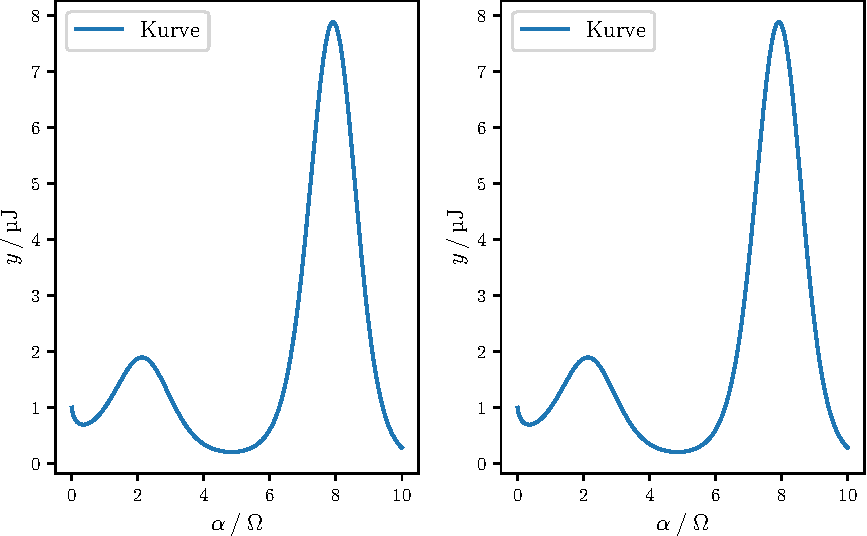
\includegraphics[width=10cm]{build/plot.pdf}
    \caption{Darstellung der Messwerte und der linearen Regression zur Bestimmung des Eigenträgheitsmoments $I_D$}
\end{figure}

\begin{table}[H]
\normalsize

\centering
\sisetup{table-format=4.0}
\begin{tabular}{c c c c}
\toprule
    $a$\,/\,$\si{\meter}$ &  $T$\,/\,$\si{\second}$ & $a^2$\,/\,$\si{\meter}^2$ &  $T^2$\,/\,$\si{\second}^2$ \\
    \midrule

0.30  &   8.35 &  0.0900      & 69.7225\\
0.285 &   7.73 &  0.0812  & 59.7529\\
0.27  &   7.65 &  0.0729    & 58.5225\\
0.255 &   7.13 &  0.0650  & 50.8369\\
0.24  &   6.83 &  0.0576    & 46.6489\\
0.225 &   6.60 &  0.0506  & 43.5600\\
0.21  &   6.40 &  0.0441    & 40.9600\\
0.195 &   5.84 &  0.0380  & 34.1056\\
0.18  &   5.24 &  0.0324    & 27.4576\\
0.165 &   5.06 &  0.0272  & 25.6036\\ 

    \bottomrule
\end{tabular}
\caption{Aufgenommene Werte zur Bestimmung des Eigenträgheitsmoments $I_{D}$ der Drillachse (Auslenkung betrug 15°)}
\label{tab:a2}
\end{table}







\subsection{Trägheitsmoment eines kurzen Zylinders}



\subsubsection{Berechung von dem Theoriewert}

Das Trägheitsmoment des ersten Zylinders, der sich um seine Symmetrieachse dreht,
($R_{K1} = 0.0375\, \si{\meter}$, $m_{K1} = 1.1193\, \si{\kilogram}$) 
lässt sich über die Gleichung \ref{eq:zyl1} ermitteln, welche den Theoriewert 
\begin{equation}
    I_{K1} = 0.787\cdot 10^{-3}\, \si{\kilogram}\,\si{\meter}^2 \nonumber
\end{equation} 
\noindent
liefert.



\subsubsection{Experimenteller Wert}

Die in Tabelle \ref{tab:a4} aufgeführten Werte wurden bei einer 
Auslenkung von $\phi = 15\,°$ aufgenommen. Mit dem, über die Gleichungen \ref{eq:fa2},
\ref{eq:ae3} und \ref{eq:std} 
errechneten, Wert $T_{K1} = 1.032 \pm 0.0463\, \si{\second}$
für die Periodendauer lässt sich über die nach $I$ umgestellte Gleichung \ref{eq:fa2}
\begin{equation}
    I = \frac{T^2 D}{4 \pi^2}
\end{equation}
und der Gaußsche Fehlerfortpflanzungformel \ref{eq:gauss}
\begin{equation} 
    \Delta I_{K1} = \sqrt{\frac{T_{K1}^2 D^2}{4 \pi^4}\Delta T_{K1}^2 + \frac{T_{K1}^4}{16 \pi^4}\Delta D^2} 
\end{equation}
\noindent
der experimentelle Wert für das Trägheitsmoment $I_{K1}$ mit
\begin{equation}
    I_{K1} = 0.00046 \pm 0.00006\, \si{\kilogram}\,\si{\meter\squared}
\end{equation}
\noindent
angeben.

\begin{table}[H]
\normalsize

\centering
\sisetup{table-format=4.0}
\begin{tabular}{c c}
\toprule
    Messung  & $T$\,/\,$\si{\second}$ \\
    \midrule

1  &   0.92   \\
2  &   1.16   \\
3  &   0.96   \\
4  &   1.12   \\
5  &   1.00   \\

    \bottomrule
\end{tabular}
\caption{Aufgenommene Werte zur Bestimmung des Trägheitsmoments $I_{K1}$}
\label{tab:a4}
\end{table}










\subsection{Trägheitsmoment eines langen Zylinders}
\subsubsection{Theoriewert}
Der Theoriewert des zweiten Zylinders 
($R_{K2} = 0.04\, \si{\meter}$, $h_{K2} = 0.1394\, \si{\meter}$, $m_{K2} = 1.5255\, \si{\kilogram}$) 
lässt sich über Gleichung \ref{eq:zyl2}
bestimmen, welche mit den angegebenen Werten
\begin{equation}
    I_{K2} = 3.1019\cdot 10^{-3}\, \si{\kilogram}\,\si{\meter\squared}
\end{equation} 
\noindent
ergibt.

\subsubsection{Experimenteller Wert}
Die in Tabelle \ref{tab:aa4} aufgeführten Werte wurden bei einer 
Auslenkung von $\phi = 15\,°$ aufgenommen. Mit dem, über die Gleichungen \ref{eq:fa2},
\ref{eq:ae3} und \ref{eq:std}, berechneten
Wert $T_{K2} = 2.032 \pm 0.0515\, \si{\second}$
für die Periodendauer lässt sich über die nach $I$ umgestellte Gleichung \ref{eq:fa2}
\begin{equation}
    I = \frac{T^2 D}{4 \pi^2}
\end{equation}
und der Gaußsche Fehlerfortpflanzungformel \ref{eq:gauss}
\begin{equation} 
    \Delta I_{K2} = \sqrt{\frac{T_{K2}^2 D^2}{4 \pi^4}\Delta T_{K2}^2 + \frac{T_{K1}^4}{16 \pi^4}\Delta D^2} 
\end{equation}
\noindent
der experimentelle Wert für das Trägheitsmoment $I_{K2}$ mit
\begin{equation}
    I_{K2} = 0.00178 \pm 0.00018\, \si{\kilogram}\,\si{\meter\squared}
\end{equation}
\noindent
angeben.

\begin{table}[H]
\normalsize

\centering
\sisetup{table-format=4.0}
\begin{tabular}{c c}
\toprule
    Messung  & $T$\,/\,$\si{\second}$ \\
    \midrule

1  &   2.23   \\
2  &   1.95   \\
3  &   2.01   \\
4  &   2.02   \\
5  &   1.95   \\

    \bottomrule
\end{tabular}
\caption{Aufgenommene Werte zur Bestimmung des Trägheitsmoments $I_{K2}$}
\label{tab:aa4}
\end{table}





\subsection{Vermessung der Holzpuppe}

Die Holzpuppe wird so betrachtet, wie es zuvor beschrieben wurde. Mithilfe der beiden 
Gleichungen
\begin{equation}
    V_{Zylinder} = \pi \cdot r^2 \cdot h 
\end{equation}
\noindent
und 
\begin{equation}
    V_{Kugel} = \frac{4}{3} \pi r^3
\end{equation}
\noindent
können die Volumina von Zylindern und Kugeln errechnet werden. Die Ergebnisse zur Vermessung der
Holzpuppe sind in Tabelle \ref{tab:zz} zu finden.

\begin{table}[H]
\normalsize

\centering
\sisetup{table-format=4.0}
\begin{tabular}{c c c}
\toprule
    Körperteil &  $r$\,/\,$\si{\meter}$ & $h$\,/\,$\si{\meter}$ \\
    \midrule

Arme        &   $6.46 \cdot 10^{-3}$   &  0.1261 \\
Beine       &   $7.07 \cdot 10^{-3}$   &  0.1484 \\
Oberkörper  &   $0.01854 $    &  0.0996 \\
Kopf        &   $0.01623 $     &  -      \\

    \bottomrule
\end{tabular}
\caption{Aufgenommene Werte zur Vermessung der Holzpuppe}
\label{tab:zz}
\end{table}
\noindent

Mit der angenommenen 
Holzdichte von $\rho = 670\,\si{\kilo\gram \per \cubic \meter}$ (siehe \cite{holz}) und der
Formel
\begin{equation}
    m = \rho \cdot V
\end{equation}
lassen sich die Massen der einzelnen Körperteile berechnen. Die einzelnen Werte der 
Massen sind ebenfalls in Tabelle \ref{tab:zz} aufgeführt.

\begin{table}[H]
\normalsize

\centering
\sisetup{table-format=4.0}
\begin{tabular}{c c c}
\toprule
    Körperteil &  $V$\,/\,$\si{\meter}^3$ & $m\,/\,\si{\kilogram}$ \\
    \midrule

$V_{Arme}$        &   $1.65322 \cdot 10^{-5}$  &  0.01108    \\
$V_{Beine}$       &   $2.33036 \cdot 10^{-5}$  &  0.01561    \\
$V_{Oberkoerper}$  &   $1.07555 \cdot 10^{-4}$  &  0.07206    \\
$V_{Kopf}$        &   $1.79079 \cdot 10^{-5}$  &  0.01200    \\

    \bottomrule
\end{tabular}
\caption{Errechnete Volumina und Massen einzelner Körperteile}
\label{tab:zz}
\end{table}



\subsection{Theoriewerte zu erster Haltung}

Über den Satz von Steiner und die Gleichungen \ref{eq:zyl1}, \ref{eq:zyl2} und \ref{eq:Kugel} 
lassen sich die theoretischen Werte der Trägheitsmomente der einzelnen
Körperteile berechnen. Die Teilergebnisse lauten:
\begin{align}
    I_{Arm} = I_{Arm,0} + (\frac{1}{2} h_{Arm}+r_{Oberkoerper})^2 m_{Arm} \nonumber \\
    I_{Arm} = 2.877 \cdot 10^{-5}\,\si[inter-unit-product=\cdot]{\kilo\gram\meter\squared} \nonumber \\
    I_{Bein} = I_{Bein,0} + (\frac{1}{2} h_{Bein}+r_{Bein})^2 m_{Bein} \nonumber \\
    I_{Bein} = 3.686 \cdot 10^{-5}\,\si[inter-unit-product=\cdot]{\kilo\gram\meter\squared} \nonumber \\
    I_{Oberkoerper} = I_{Oberkoerper,0}\nonumber \\
    I_{Oberkoerper} = 1.228 \cdot 10^{-5}\,\si[inter-unit-product=\cdot]{\kilo\gram\meter\squared} \nonumber \\
    I_{Kopf} = I_{Kopf,0}\nonumber \\
    I_{Kopf} = 1.253 \cdot 10^{-6}\,\si[inter-unit-product=\cdot]{\kilo\gram\meter\squared} \nonumber \\
\end{align}
\noindent
Werden all diese Teilergebnisse aufsummiert, ergibt sich das insgesamte Trägheitsmoment 
\begin{equation}
    I_{Position,1} = 7.916 \cdot 10^{-5}\,\si[inter-unit-product=\cdot]{\kilo\gram\meter\squared}
\end{equation}
der Holzpuppe in der ersten
Haltung.


\subsection{Experimentell bestimmter Wert des Trägheitsmoments}

In diesem Teil kann das Trägheitsmoment analog zu der Berechnung der beiden Trägheitsmomente $I_{K1}$
und $I_{K2}$ erfolgen. 
Die in Tabelle \ref{tab:euler} aufgeführten Werte wurden bei einer 
Auslenkung von $\phi = 20\,°$ aufgenommen. Mit dem, über die Gleichungen \ref{eq:fa2}, \ref{eq:ae3} 
und \ref{eq:std} errechneten, 
Wert $T_{P,1} = 0.8220 \pm 0.0285\, \si{\second}$
für die Periodendauer lässt sich über die nach $I$ umgestellte Gleichung \ref{eq:fa2}
\begin{equation}
    I = \frac{T^2 D}{4 \pi^2}
\end{equation}
und der Gaußsche Fehlerfortpflanzungformel \ref{eq:gauss}
\begin{equation} 
    \Delta I_{Position,1} = \sqrt{\frac{T_{P,1}^2 D^2}{4 \pi^4}\Delta T_{P,1}^2 + \frac{T_{P,1}^4}{16 \pi^4}\Delta D^2} 
\end{equation}
\noindent
der experimentelle Wert für das Trägheitsmoment $I_{Position,1}$ mit
\begin{equation}
    I_{Position,1} = 0.000291 \pm 0.000033\, \si{\kilogram}\,\si{\meter\squared}
\end{equation}
\noindent
angeben.

\begin{table}[H]
\normalsize

\centering
\sisetup{table-format=4.0}
\begin{tabular}{c c}
\toprule
    Messung  & $T$\,/\,$\si{\second}$ \\
    \midrule

1  &   0.73   \\
2  &   0.86   \\
3  &   0.87   \\
4  &   0.87   \\
5  &   0.78   \\

    \bottomrule
\end{tabular}
\caption{Aufgenommene Werte zur Bestimmung des Trägheitsmoments}
\label{tab:euler}
\end{table}



\subsection{Theoriewerte zu zweiter Haltung}

Über den Satz von Steiner und die Gleichungen \ref{eq:zyl1}, \ref{eq:zyl2} und \ref{eq:Kugel} 
lassen sich die theoretischen Werte der Trägheitsmomente der einzelnen
Körperteile berechnen. Die Teilergebnisse lauten:
\begin{align}
    I_{Arm} = I_{Arm,0} + (r_{Oberkoerper})^2 m_{Arm} \nonumber \\
    I_{Arm} = 1.926 \cdot 10^{-6}\,\si[inter-unit-product=\cdot]{\kilo\gram\meter\squared}\nonumber \\
    I_{Bein} = I_{Bein,0} + (r_{Bein})^2 m_{Bein} \nonumber \\
    I_{Bein} = 4.583 \cdot 10^{-7}\,\si[inter-unit-product=\cdot]{\kilo\gram\meter\squared}\nonumber \\
    I_{Oberkoerper} = I_{Oberkoerper,0}\nonumber \\
    I_{Oberkoerper} = 1.228 \cdot 10^{-5}\,\si[inter-unit-product=\cdot]{\kilo\gram\meter\squared}\nonumber \\
    I_{Kopf} = I_{Kopf,0}\nonumber \\
    I_{Kopf} = 1.253 \cdot 10^{-6}\,\si[inter-unit-product=\cdot]{\kilo\gram\meter\squared}\nonumber \\
\end{align}

\noindent
werden all diese Teilergebnisse aufsummiert, ergibt sich das insgesamte Trägheitsmoment 
\begin{equation}
    I_{Position,2} = 1.591 \cdot 10^{-5}\,\si[inter-unit-product=\cdot]{\kilo\gram\meter\squared} 
\end{equation}
der Holzpuppe in der zweiten
Haltung.



\subsection{Experimentell bestimmter Wert des Trägheitsmoments}
 
Die in Tabelle \ref{tab:furlan} aufgeführten Werte wurden bei einer 
Auslenkung von $\phi = 20\,°$ aufgenommen. Mit dem, über die Gleichungen \ref{eq:fa2}, \ref{eq:ae3} und \ref{eq:std} errechneten, 
Wert $T_{P,2} = 0.382 \pm 0.0242\, \si{\second}$
für die Periodendauer lässt sich über die nach $I$ umgestellte Gleichung \ref{eq:fa2}
\begin{equation}
    I = \frac{T^2 D}{4 \pi^2}
\end{equation}
und der Gaußsche Fehlerfortpflanzungformel \ref{eq:gauss}
\begin{equation} 
    \Delta I_{P,2} = \sqrt{\frac{T_{P,2}^2 D^2}{4 \pi^4}\Delta T_{P,2}^2 + \frac{T_{P,2}^4}{16 \pi^4}\Delta D^2} 
\end{equation}
\noindent
der experimentelle Wert für das Trägheitsmoment $I_{K2}$ mit
\begin{equation}
    I_{Position,2} = (6.3 \pm 1.0)10^{-5}\, \si{\kilogram}\,\si{\meter\squared}
\end{equation}
\noindent
angeben.

\begin{table}[H]
\normalsize

\centering
\sisetup{table-format=4.0}
\begin{tabular}{c c}
\toprule
    Messung  & $T$\,/\,$\si{\second}$ \\
    \midrule

1  &   0.46   \\
2  &   0.36   \\
3  &   0.32   \\
4  &   0.41   \\
5  &   0.36   \\

    \bottomrule
\end{tabular}
\caption{Aufgenommene Werte zur Bestimmung des Trägheitsmoments}
\label{tab:furlan}
\end{table}





\begin{equation*}
  I=0,787 \cdot 10^{-3}\,\si[inter-unit-product=\cdot]{\kilo\gram\meter\squared}
\end{equation*}
\begin{equation*}
  I=15,432 \cdot 10^{-3}\,\si[inter-unit-product=\cdot]{\kilo\gram\meter\squared}
\end{equation*}
\begin{equation*}
  I=7,916 \cdot 10^{-5}\,\si[inter-unit-product=\cdot]{\kilo\gram\meter\squared}
\end{equation*}
\begin{equation*}
  I=1,591 \cdot 10^{-5}\,\si[inter-unit-product=\cdot]{\kilo\gram\meter\squared}
\end{equation*}